\subsubsection{} \textit{RSA} шифровка и расшифровка.
\label{sec:eng:performance:rsaenc}

Метод \texttt{rsaEncrypt} необходим для зашифровки данных при помощи алгоритма \textit{RSA}, а метод \texttt{rsaDecrypt} -- для расшифровки данных, зашифрованных при помощи \textit{RSA}. На рисунках \ref{sec:eng:performance:rsaenc:enc} и \ref{sec:eng:performance:rsaenc:dec} результаты измерений генерации \textit{RSA} и \textit{AES} ключей соответственно.

\begin{figure}[h]
\centering
\begin{minipage}{.5\textwidth}
  \centering
  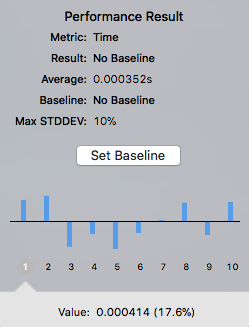
\includegraphics[width=.65\linewidth]{inc/img/perf/testRSAEncryptPerformance.png}
  \captionof{figure}{Результаты замеров шифровки при помощи RSA}
  \label{sec:eng:performance:rsaenc:enc}
\end{minipage}%
\begin{minipage}{.5\textwidth}
  \centering
  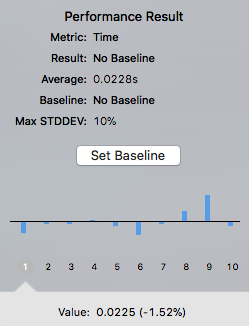
\includegraphics[width=.65\linewidth]{inc/img/perf/testRSADecryptPerformance.png}
  \captionof{figure}{Результаты замеров дешифровки при помощи RSA}
  \label{sec:eng:performance:rsaenc:dec}
\end{minipage}
\end{figure}

\FPeval{\rsaEncMesaureMax}{0.00423}
\FPeval{\rsaEncMesaureMin}{0.00281}
\FPeval{\rsaEncMesaureAverage}{0.00352}
\FPeval{\perfRSAEnc}{clip(round(((\rsaEncryptMaxValue - (\rsaEncMesaureMax + \rsaEncMesaureMin + \rsaEncMesaureAverage) / 3) / \rsaEncryptMaxValue) * 100, 2))}

Рассчитаем отклонение от предельно допустимого значения времени, затраченного на шифрование при помощи \textit{RSA}, подставив значения в формулу (\ref{perfDifEquation}):
\begin{center}
\(\perfDev = (\num{\rsaEncryptMaxValue} - \frac{\num{\rsaEncMesaureMax} + \num{\rsaEncMesaureMin} + \num{\rsaEncMesaureAverage}}{\num{3}}) \cdot \frac{\num{1}}{\num{\rsaEncryptMaxValue}} \cdot 100 = \num{\perfRSAEnc} \, \text{\%}\)
\end{center}

\FPeval{\rsaDecMesaureMax}{0.236}
\FPeval{\rsaDecMesaureMin}{0.224}
\FPeval{\rsaDecMesaureAverage}{0.228}
\FPeval{\perfRSADec}{clip(round(((\rsaDecryptMaxValue - (\rsaDecMesaureMax + \rsaDecMesaureMin + \rsaDecMesaureAverage) / 3) / \rsaDecryptMaxValue) * 100, 2))}

Для дешифровки, при помощи алгоритма \textit{RSA}, рассчитаем аналогичное значение:
\begin{center}
\(\perfDev = (\num{\rsaDecryptMaxValue} - \frac{\num{\rsaDecMesaureMax} + \num{\rsaDecMesaureMin} + \num{\rsaDecMesaureAverage}}{\num{3}}) \cdot \frac{\num{1}}{\num{\rsaDecryptMaxValue}} \cdot 100 = \num{\perfRSADec} \, \text{\%}\)
\end{center}